\documentclass[a4paper,10.5pt]{jsarticle}

% 数式
\usepackage{amsmath,amsfonts}
\usepackage{amsthm}
\usepackage{bm}
\usepackage{mathtools}
\usepackage{amssymb}

% 表
\usepackage[utf8]{inputenc}
\usepackage{diagbox} % 斜線付きセルを作成するために必要
\usepackage{booktabs} % 表の罫線を美しくするために必要
\usepackage{hhline} % 水平罫線を制御するために必要

% 画像
\usepackage[dvipdfmx]{graphicx}
\usepackage{ascmac}
\usepackage{physics}
\usepackage{float} % 追加

% 図
\usepackage[dvipdfmx]{graphicx}
\usepackage{tikz} %図を描く
\usetikzlibrary{positioning, intersections, calc, arrows.meta,math} %tikzのlibrary

% ハイパーリンク
\usepackage[dvipdfm,
  colorlinks=false,
  bookmarks=true,
  bookmarksnumbered=false,
  pdfborder={0 0 0},
  bookmarkstype=toc]{hyperref}

% 式番号を章ごとにリセット
\numberwithin{equation}{section}

\begin{document}

\title{15章}
\author{大上由人}
\date{\today}
\maketitle
\setcounter{section}{14}

\section{最大仕事率のもとでのエンジンの効率}
有限時間における熱力学を考える。従来の熱力学において、熱機関の最高効率はカルノーサイクルによって達成され、以下のように表される。
\begin{align}
  \eta_{\text{C}} = 1 - \frac{T_{\text{L}}}{T_{\text{H}}}
\end{align}
ただし、$T_{\text{L}}$は低温熱浴の温度、$T_{\text{H}}$は高温熱浴の温度である。しかし、この効率は、どの操作も準静的に行うため、1サイクル回すのには無限の時間がかかる。
したがって、この熱機関の仕事率は0となってしまう。現実の世界に熱機関を適応するうえでは仕事率もある程度高くあってほしい。そこで、この章では、仕事率を最大にしたときの効率について考える。とくに、サイクルを回すのにかかる時間は有限である。

\subsection{エンドリバーシブル過程とカーゾン-アルボーン効率}
\begin{itembox}[l]{\textbf{Def. Endoreversible 熱力学}}
  Endoreversible熱力学とは、温度$T$の熱浴に接触した等温過程で、以下の性質を満たすものである。
  \begin{itemize}
    \item 系は常に平衡状態にある。その温度$T'$は熱浴の温度$T$と異なる可能性もある。
    \item 系と熱浴の熱交換は、Fourierの法則に従う。すなわち、
    \begin{equation}
      J_{Q} = \kappa(T-T')
    \end{equation}
    ただし、$J_{Q}$は系に入ってくる向きの熱流、$\kappa$は熱コンダクタンスである。
    \item 系の温度$T'$はその系のエネルギー$E$,体積$V$,粒子数$N$の組$(E,V,N)$にのみ依存する。
  \end{itemize}
\end{itembox}

\begin{figure}[H]
    \begin{center}
    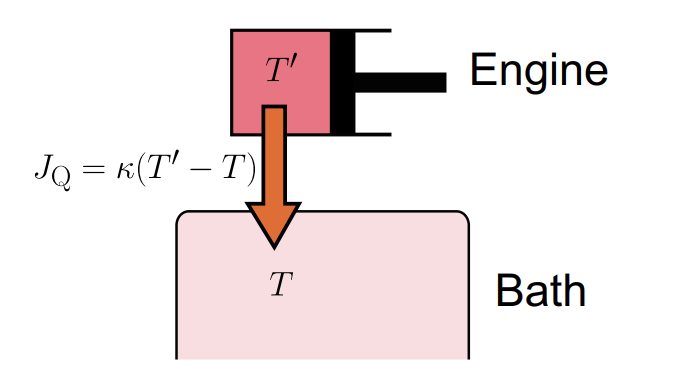
\includegraphics[width=100mm]{endoreversible.png}
    \end{center}
    \caption{Endoreversible熱力学の模式図}
    \label{fig:endoreversible}
\end{figure}

この枠組みでの熱機関のサイクル過程を考える。この過程において、系は高温熱浴(温度$T_{H}$)と低温熱浴(温度$T_{L}$)との間でエネルギーをやり取りする。
我々は、断熱過程は可逆であるが、等温過程に比べて圧倒的に素早く行われると仮定する。また、等温過程において、高温(低温)熱浴と接しているとき、系の温度は$T'_H$($T'_L$)で一定であると仮定する。このとき、
以下の定理を示すことができる。

\begin{itembox}[l]{\textbf{Thm.Curzon-Ahlborn 効率}}
  すべての物質特性(熱コンダクタンス、エントロピー関数など)が固定されていて、熱機関の二つの温度$T'_H$と$T'_L$が制御可能なパラメータであると仮定する。このとき、
  最大仕事率の元での熱機関の効率は以下の不等式を満たす。
  \begin{equation}
    \eta_{\text{MP}} \leq 1 - \sqrt{\frac{T_L}{T_H}} := \eta_{\text{CA}}
  \end{equation}
  この最右辺の値をCurzon-Ahlborn効率という。\footnote{$\eta_{\text{MP}}$は最大仕事率の元での効率を表す。}
\end{itembox}
\textbf{Prf.}\\
$Q_{H}$を高温熱浴から系に流れ込む熱量、$Q_{L}$を系から低温熱浴に流れ出る熱量とする。また、高温(低温)熱浴と接している時間をそれぞれ$t_{H}$($t_{L}$)とする。また、それぞれの熱コンダクタンスを$\kappa_{H}$($\kappa_{L}$)とする。このとき、
\begin{align}
  Q_{H} &= \kappa_{H}t_{H}(T_{H}-T'_{H})\\
  Q_{L} &= \kappa_{L}t_{L}(T'_{L}-T_{L})
\end{align}
となる。また、サイクル全体でエントロピーが変化しないことから、高温熱浴との相互作用でのエントロピー増大と、低温熱浴との相互作用でのエントロピー減少が等しい。すなわち、
\begin{equation}
  \Delta S = \frac{Q_{H}}{T'_{H}} = \frac{Q_{L}}{T'_{L}}
\end{equation}
となる。このとき、仕事率は、断熱過程にかかる時間を十分小さいとして、
\begin{align}
  \dot{W} &= \frac{Q_{H} - Q_{L}}{t_{H} + t_{L}}
\end{align}
$x = T_{H} - T'_{H},\quad y = T'_{L} - T_{L}$とすると、
\begin{align}
  Q_{H} &= \kappa_{H}t_{H}(T_{H}-T'_{H}) = \kappa_{H}t_{H}x\\
  Q_{L} &= \kappa_{L}t_{L}(T'_{L}-T_{L}) = \kappa_{L}t_{L}y
\end{align}
である。したがって、
\begin{align}
  t_{H} = \frac{Q_{H}}{\kappa_{H}x},\quad t_{L} = \frac{Q_{L}}{\kappa_{L}y}
\end{align}
である。これを代入すると、
\begin{align}
  \dot{W} &= \frac{Q_{H} - Q_{L}}{\frac{Q_{H}}{\kappa_{H}x} + \frac{Q_{L}}{\kappa_{L}y}}\\
  &= \frac{1-\frac{Q_{L}}{Q_{H}}}{\frac{1}{\kappa_{H}x} + \frac{1}{\kappa_{L}y\frac{Q_{L}}{Q_{H}}}}\\
  &= \frac{1-\frac{T_{L}'}{T_{H}'}}{\frac{1}{\kappa_{H}x} + \frac{1}{\kappa_{L}y\frac{T_{L}'}{T_{H}'}}}\\
  &= \frac{1-\frac{T_{L}+y}{T_{H}-x}}{\frac{1}{\kappa_{H}x} + \frac{1}{\kappa_{L}y\frac{T_{L}+y}{T_{H}-x}}}\\
  &= \frac{\kappa_{H}\kappa_{L}xy(T_{H}-x)-\kappa_{H}\kappa_{L}xy(T_{L}+y)}{\kappa_{L}y(T_{H}-x)+\kappa_{H}x(T_{L}+y)}\\
  &= \frac{(T_H + T_L - x - y)\kappa_H \kappa_L xy}{\kappa_L T_H y + \kappa_H T_L x + (\kappa_H - \kappa_L) xy}
\end{align}
となる。
これを最大化するために、$\dot{W}$を$x$と$y$で偏微分し、それが0になる条件を求めると、かなり面倒な計算の末、
\begin{align}
  \kappa_L T_H y^*(T_H + T_L - x^* - y^*) - (\kappa_L T_H y^* + \kappa_H T_L x^* + (\kappa_H - \kappa_L) x^* y^*) x^* &= 0\\
  \kappa_H T_L x^*(T_H + T_L - x^* - y^*) - (\kappa_L T_H y^* + \kappa_H T_L x^* + (\kappa_H - \kappa_L) x^* y^*) y^* &= 0
\end{align}
となる。両辺割り算して整理することで、
\begin{equation}
  y^* = \sqrt{\frac{\kappa_H T_L}{\kappa_L T_H}}x^*
\end{equation}
となる。したがって、
\begin{align}
  x^* &= \frac{T_H \left(1 - \sqrt{\frac{T_L}{T_H}} \right)}{1 + \sqrt{\frac{\kappa_H}{\kappa_L}}}\\
  y^* &= \frac{T_L \left(\sqrt{\frac{T_H}{T_L}} - 1\right)}{1 + \sqrt{\frac{\kappa_L}{\kappa_H}}}
\end{align}
このもとで、熱効率を求めると、
\begin{align}
  \eta_{\text{MP}} &= \frac{Q_H - Q_L}{Q_H} = 1 - \frac{T_L + y^*}{T_H + x^*} = 1 - \frac{T_L \sqrt{\kappa_H} \sqrt{\frac{T_H}{T_L}} + \sqrt{\kappa_L}}{T_H \sqrt{\kappa_L} \sqrt{\frac{T_L}{T_H}} + \sqrt{\kappa_H}} = 1 - \sqrt{\frac{T_L}{T_H}}
\end{align}
となる。このことと、一般にカルノーサイクルが効率最大のサイクルであることから、目的の不等式が得られる。\qed\\
(計算)\\
\begin{align}
  1-\frac{T_{L}+y}{T_{H}-x} &= 1-\frac{T_L + \frac{T_{L}\qty(\sqrt{\frac{T_{H}}{T_{L}}}-1)}{1+\sqrt{\frac{\kappa_{L}}{\kappa_{H}}}}}{T_H - \frac{T_H\qty(1-\sqrt{\frac{T_{H}}{T_{L}}})}{1+\sqrt{\frac{\kappa_{H}}{\kappa_{L}}}}}\\
  &= 1-\frac{T_L}{T_H} \frac{\sqrt{\frac{T_H}{T_L}} + \sqrt{\frac{\kappa_{L}}{\kappa_{H}}}}{\sqrt{\frac{T_L}{T_H}} + \sqrt{\frac{\kappa_{H}}{\kappa_{L}}} } \frac{1 + \sqrt{\frac{\kappa_{H}}{\kappa_{L}}}}{1 + \sqrt{\frac{\kappa_{L}}{\kappa_{H}}}}\\
  &= 1 - \frac{T_L \sqrt{\kappa_H} \sqrt{\frac{T_H}{T_L}} + \sqrt{\kappa_L}}{T_H \sqrt{\kappa_L} \sqrt{\frac{T_L}{T_H}} + \sqrt{\kappa_H}}
\end{align}


\subsection{Onsagar行列によるアプローチ}
時間反転対称性を持つような定常系を考える。\\
\textbf{記号}
\begin{itemize}
  \item \( X_1 \) :$J_{2}$によって駆動される熱力学的な力(エントロピーの自然な変数)
  \item \( X_2 \) :二つの熱浴の逆温度差
  \begin{align}
      X_2 := \frac{1}{T_L} - \frac{1}{T_H}
  \end{align}
  
  \item \( J_1 \) :熱流 \( X_1 \) に対応)
  \item \( J_2 \) :熱流(二つの熱浴の間で流れる)
  
  \item \( T_H \) :高温側の熱浴の温度
  \item \( T_L \) :低温側の熱浴の温度
  \item \( T \) :\( T_H \) と \( T_L \) が近い場合の平均温度
  (線形応答体制では \( T_L \approx T_H \approx T \) と仮定)
  
  \item パワー \( \dot{W} \) :次のように定義される
  \begin{align}
      \dot{W} := - X_1 J_1 T
  \end{align}
  
  \item 効率 \( \eta \) :次のように定義される
  \begin{align}
      \eta := - \frac{X_1 J_1 T}{J_2}
  \end{align}
  
  \item カルノー効率 \( \eta_C \)
  \begin{align}
      \eta_C := 1 - \frac{T_L}{T_H} = \frac{\Delta T}{T} 
  \end{align}
  ここで、\( \Delta T := T_H - T_L \)
\end{itemize}


線形応答理論を適応するため、揺動散逸定理のあたりで出てきたOnsagar行列を用いる。この行列は、
\begin{align}
    J_1 &= L_{11} X_1 + L_{12} X_2\\
    J_2 &= L_{21} X_1 + L_{22} X_2
\end{align}
ただし、Onsagarの相反定理により、$L_{12} = L_{21}$である。また、このとき、熱力学第二法則から、
\begin{align}
    \dot{S} := J_1 X_1 + J_2 X_2 \geq 0
\end{align}
が得られる。この不等式は、
\begin{align}
  L_{11} X_1^2 + 2L_{12} X_1 X_2 + L_{22} X_2^2 \geq 0
\end{align}
に等しい。これが常に成り立つ条件は、判別式を考えることにより、
\begin{align}
    L_{11} &\geq 0,  \\
    L_{22} &\geq 0,  \\
    L_{11}L_{22} - L_{12}^2 &\geq 0
\end{align}
となる。とくに、三本目の不等式は、
\begin{align}
    q := \frac{L_{12}}{\sqrt{L_{11}L_{22}}}
\end{align}
が
\begin{align}
  -1 \leq q \leq 1
\end{align}
を満たすことを意味する。このもとで、熱効率が以下の不等式を満たすことが知られている。

\begin{itembox}[l]{\textbf{Thm.線形応答の範囲での定常系の効率}}
  上で述べたような系について、Onsagar行列および$X_2$が固定されていて、$X_1$が制御可能なパラメータであると仮定する。このとき、最大仕事率のもとでの熱機関の効率は以下の不等式を満たす。
  \begin{align}
    \eta_{\text{MP}} \leq \frac{\eta_C}{2} 
  \end{align}
  ただし、$\eta_C$はカルノーサイクルの効率である。
\end{itembox}

\textbf{Prf.}\\
いま、仕事率は、
\begin{align}
  \dot{W} &= -X_1 J_1 T =-X_1(L_{11} X_1 + L_{12} X_2) T = \left(-L_{11} \left( X_1 + \frac{L_{12} X_2}{2 L_{11}} \right)^2 + \frac{L_{12}^2 X_2^2}{4 L_{11}} \right) T
\end{align}
と書くことができる。これは$X_1 = -L_{12} X_2 / 2 L_{11}$において最大値をとる。これを熱効率の定義に代入することで、
\begin{align}
  \eta_{\text{MP}} &= -\frac{X_1(L_{11} X_1 + L_{12} X_2) T}{L_{21} X_1 + L_{22} X_2} \\
  &= -\frac{X_1(L_{11}\qty(-\frac{L_{12} X_2}{2 L_{11}}) + L_{12} X_2) T}{L_{21} \qty(-\frac{L_{12} X_2}{2 L_{11}}) + L_{22} X_2} \\
  &= -\frac{X_1\qty(-\frac{L_{12}}{2}+ L_{12})T}{-\frac{L_{12}^2}{2L_{11}} + L_{22}} \\
  &= \frac{L_{12} X_2}{2 L_{11} }\frac{\frac{1}{2}L_{12}T}{-\frac{L_{12}^2}{2L_{11}} + L_{22}} \\
  &= \frac{L_{12} X_2}{2 L_{11} }\frac{\frac{L_{12}}{L_{22}}T}{2-\frac{L_{12}^2}{L_{11}L_{22}} } \\
  &= \frac{1}{2} \frac{L_{12}^2}{L_{11}L_{22}} \frac{T}{2-q^2}X_2\\
  &\simeq \frac{1}{2} \frac{\Delta T}{T} \frac{q^2}{2 - q^2} \\
  &\leq \frac{1}{2} \frac{\Delta T}{T}\\
  &= \frac{\eta_C}{2}
\end{align}
したがって、目的の不等式が得られる。\qed\\
このセットアップの偉いところは、Curzon-Ahlbornのセットアップとは異なり、線形応答の範囲の定常系であれば適応できる点である。
ただし、Curzon-Ahlbornのセットアップの方が良いところもある。それは、Curzon-Ahlbornのセットアップは、系と熱浴の温度差が小さいと仮定しているだけであり、熱浴の温度差については仮定していない点である

\subsection{速度による展開}
外部から制御できる唯一のパラメータとして、操作速度$u$を導入する。ここでは、高温熱浴と低温熱浴での等温過程の操作速度の比が一定であると仮定する。
\begin{itembox}[l]{\textbf{Thm.}}
外部から操作される熱機関を考える。その動作速度はパラメータ $u$ によって特徴付けられ、この $u$ は操作可能なパラメータとする。熱機関が $u \to 0$ の極限で最大効率 $\eta_{\text{max}}$ を達成すると仮定する。
また、各カレントに伴う単位時間あたりの散逸量は $u$ の増加に伴って増加するものと仮定する。すると、$u$ に関して線形応答の範囲内では、
\begin{align}
    \frac{\eta_{\text{max}}}{2} \leq \eta_{\text{MP}} \leq \frac{1}{2 - \eta_{\text{max}}}
\end{align}
が小さい $u$ の場合に成立する。
\end{itembox}

特に、線形応答の範囲内(すなわち、2つの熱浴間の温度差が小さい場合)では、
\begin{align}
    \eta_{\text{MP}} = \frac{\eta_{\text{max}}}{2}
\end{align}
が成立する。また、Curzon-Ahlborn効率 $\eta_{\text{CA}} := 1 - \sqrt{\frac{T_L}{T_H}}$ は $\eta_{\text{max}} = 1 - \frac{T_L}{T_H}$ を用いて式(15.22)を満たす。

\textbf{Prf.} $J_Q,J_W$ をそれぞれ高温熱浴からの熱流と単位時間あたりに取り出される仕事量とする。$J_W$ と $J_Q$ を $u$ で展開する:
\begin{align}
    J_W(u) &= a_1 u - a_2 u^2 + \cdots \\
    J_Q(u) &= b_1 u - b_2 u^2 + \cdots
\end{align}

ただし、$u \to 0$でカレントが0になるため、定数項は現れない。効率が準静的な極限で最大効率 $\eta_{\text{max}}$ に近づくため、以下が成り立つ:
\begin{align}
    \frac{a_1}{b_1} = \eta_{\text{max}}
\end{align}

仕事の取り出しにおける散逸項 $a_2 u^2$ は、低温熱浴への熱流における対応する散逸項である $b_2 u^2$ と等しいため、$a_2 \geq b_2 \geq 0$ が成立する。
%TODO怪しい

今、仕事率$J_W$は、
\begin{align}
    u^* = \frac{a_1}{2 a_2}
\end{align}
において最大化される。このとき、効率は
\begin{align}
    \eta_{\text{MP}} := \frac{J_W(u^*)}{J_Q(u^*)} &= \frac{a_1 - a_2 \frac{a_1}{2a_2}}{b_1 \left( 1 - \frac{b_2}{b_1} \frac{a_1}{2a_2} \right)} = \frac{\eta_{\text{max}}}{2} \frac{1}{1 - \eta_{\text{max}} \frac{b_2}{2a_2}}
\end{align}
$\mathcal{O}(u^*)$ まで。この式に $0 \leq \frac{b_2}{a_2} \leq 1$ を代入すると、所望の不等式(15.22)が得られる。 \hfill $\Box$

ここで2つの注意を述べる。まず、もし高温熱浴からの熱流の損失と低温熱浴への損失が等しい場合、$a_2 = 2 b_2$ が成立し、この場合のEMPは次のように書ける
\begin{align}
    \eta_{\text{MP}} := \frac{\eta_{\text{max}}}{2} \frac{1}{1 - \frac{\eta_{\text{max}}}{4}} = \frac{\eta_{\text{max}}}{2} + \frac{\eta_{\text{max}}^2}{8} + {O}(\eta_{\text{max}}^3)
\end{align}

この式は、左右対称性を持つ普遍的な2次の係数 $1/8$ を回復する。

次に、最大効率がカルノー効率 $\eta_{\text{max}} = \eta_C$ であると仮定していない点に留意する。
上述の定理は、一般的に、準静的極限 $u \to 0$ で熱の散逸がない場合、EMPが最大効率の半分に等しいことを示している。したがって、有限サイズの熱浴を持つ熱機関にこの定理を適用すると、たとえば、エクセルギーに関してEMPが効率の半分であることが示される。

\end{document}